% Using pdfpages strips all links from the pdfs. There is a package called pax that restores some (all?) of the links. Check it out if you have the time.
\part{Papers}
\label{part:papers}

\appendix
% Hack the "Chapter" names
%\newcommand{\appchapter}[1]{\let\oldthechapter\thechapter
%  \renewcommand{\thechapter}{Paper \oldthechapter}
%    \chapter{#1}\let\thechapter\oldthechapter}

%\appchapter{Hydrogen Rotational and Translational Diffusion in Calcium Borohydride from Quasielastic Neutron Scattering and DFT Calculations}
%\label{pap:calcium}
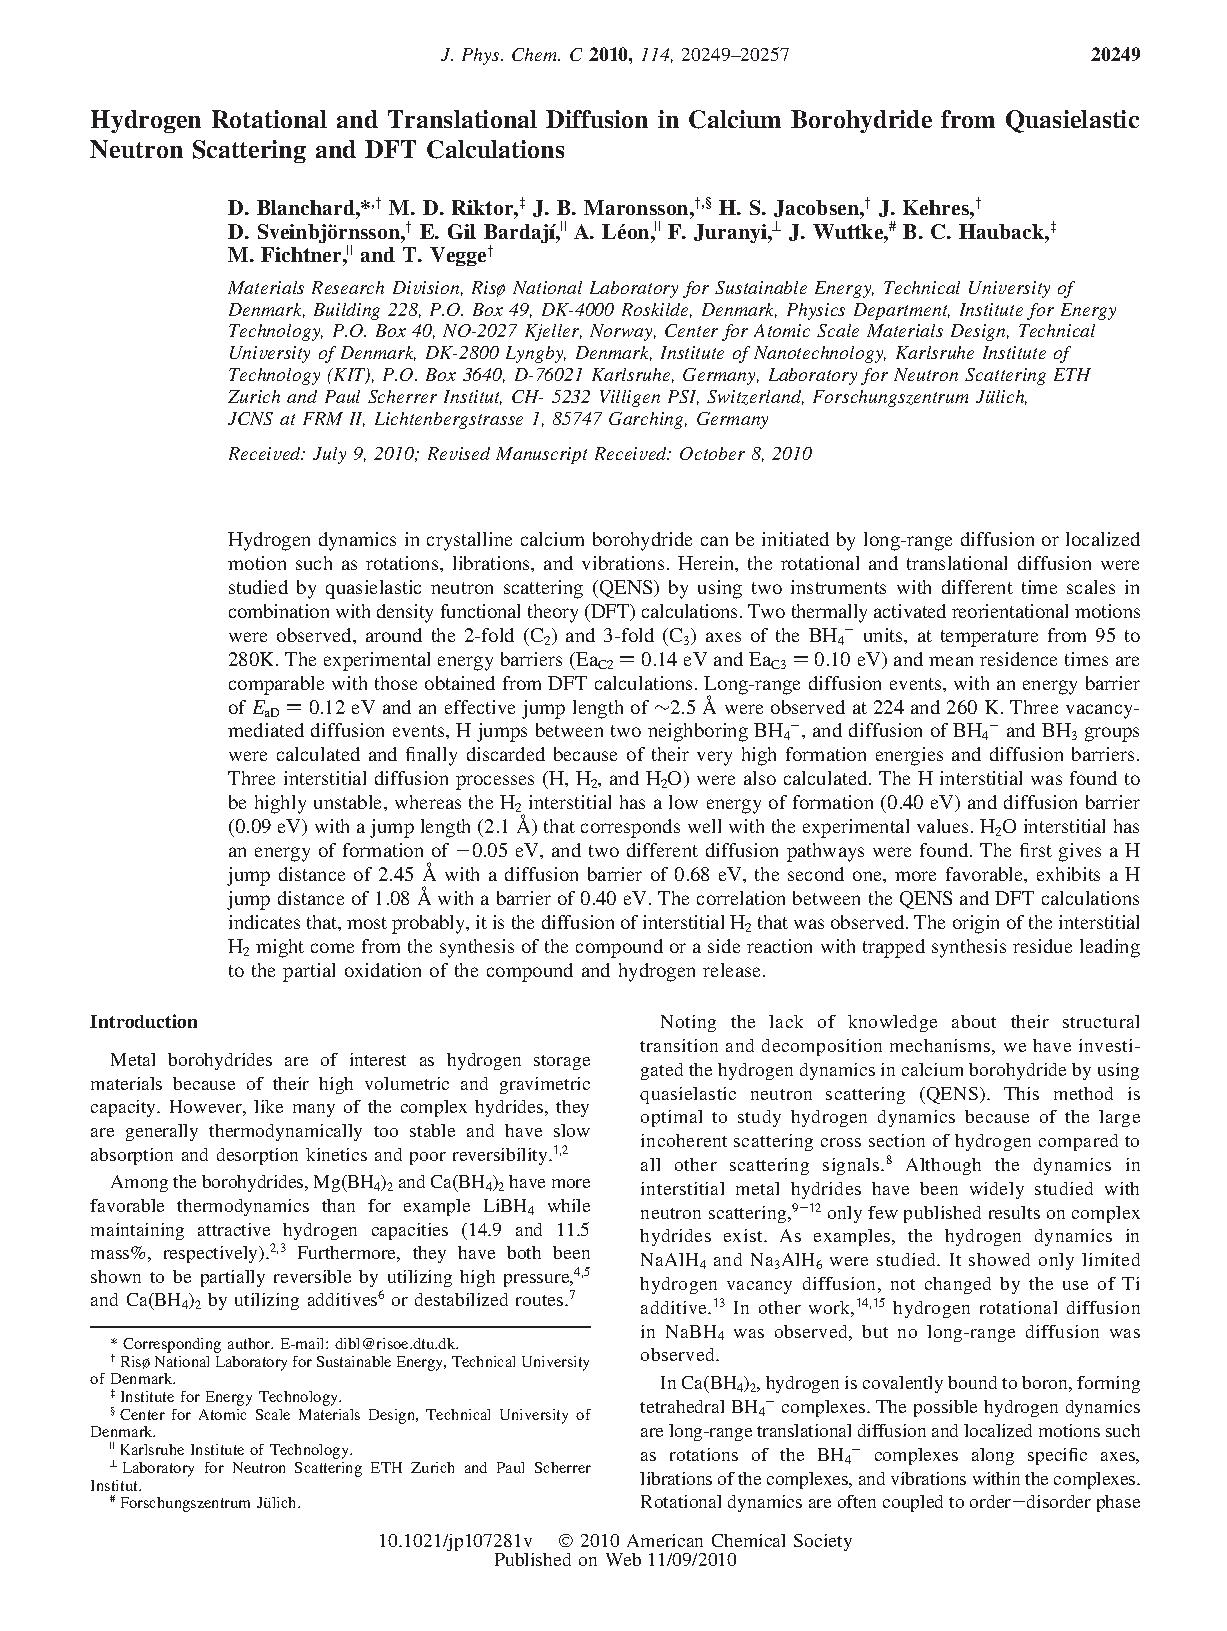
\includepdf[pages=1, addtotoc={1,chapter,0,Hydrogen Rotational and Translational Diffusion in Calcium Borohydride from Quasielastic Neutron Scattering and DFT Calculations,pap:calcium}]{papers/calcium.pdf}
%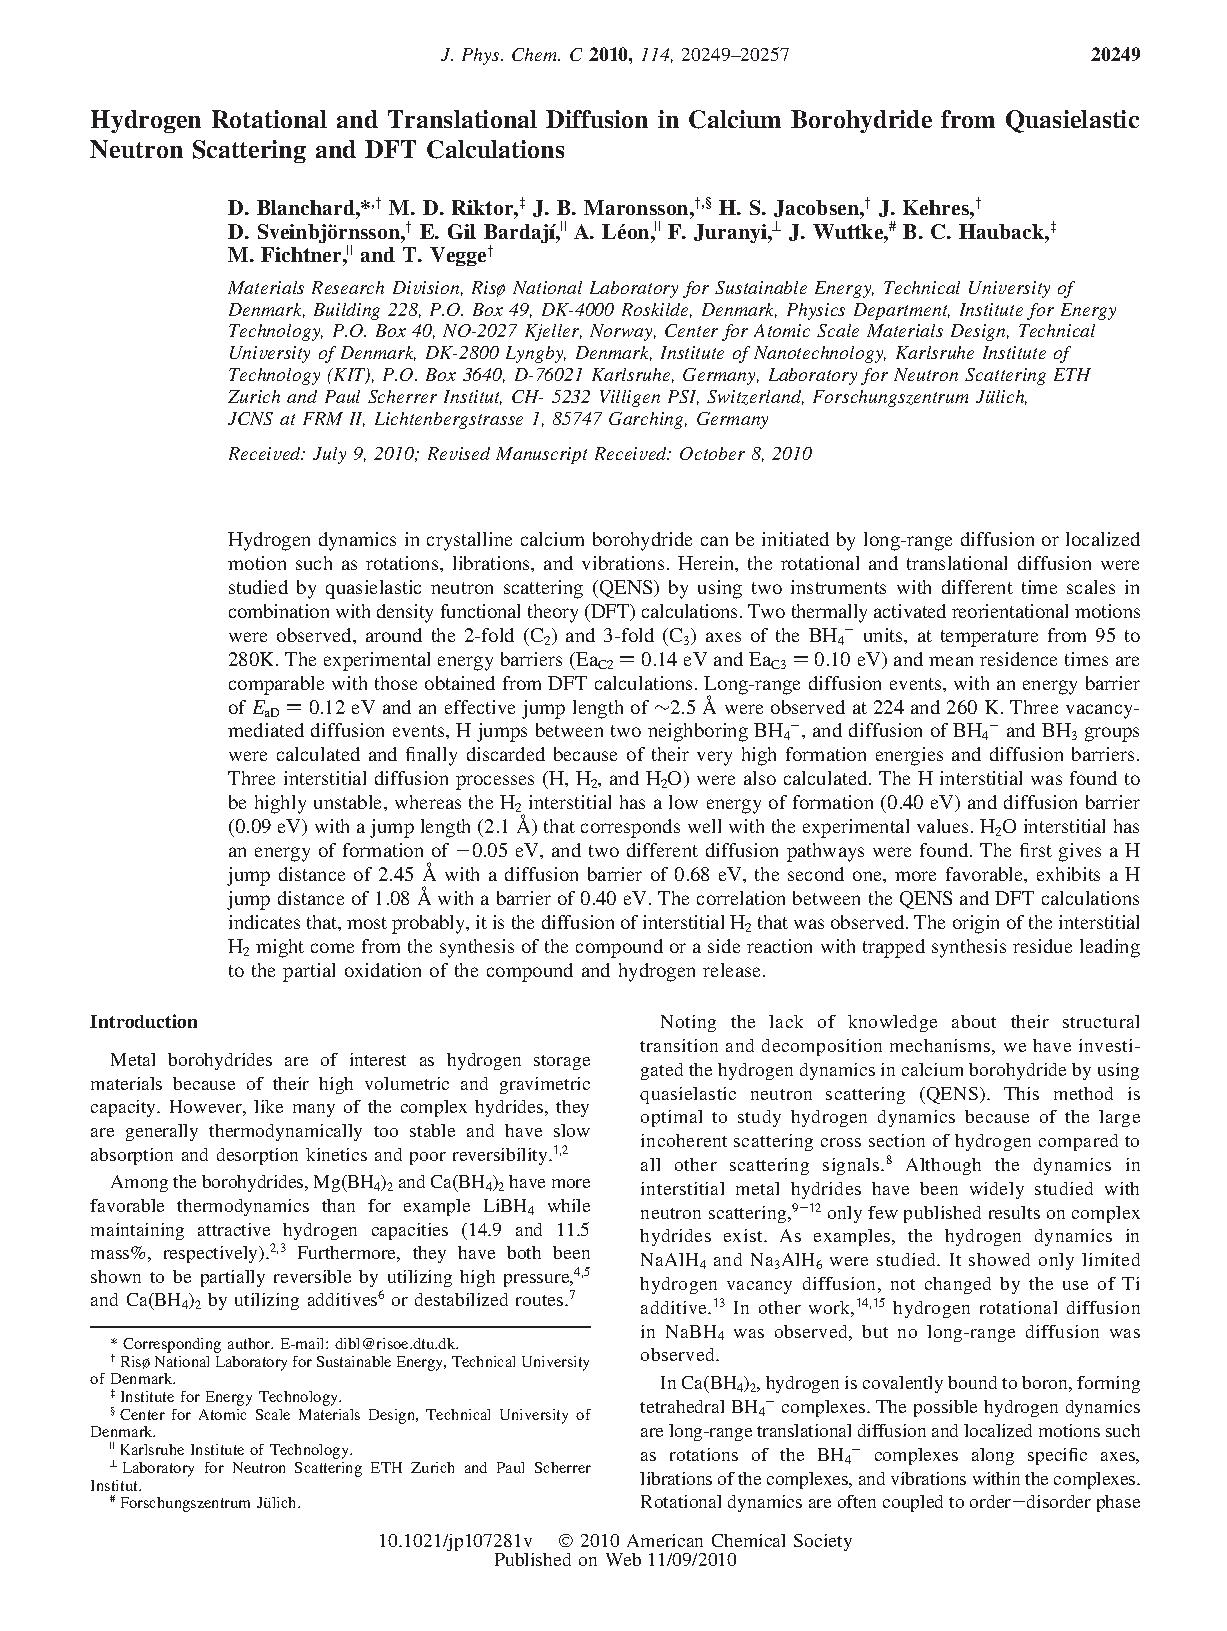
\includepdf[pages=-, openright, fitpaper, addtotoc={1,chapter,0,Hydrogen Rotational and Translational Diffusion in Calcium Borohydride from Quasielastic Neutron Scattering and DFT Calculations,pap:calcium}]{papers/calcium.pdf}

%\appchapter{Hindered Rotational Energy Barriers of \ce{BH4-} Tetrahedra in $\beta$-\ce{Mg(BH4)2} from Quasielastic Neutron Scattering and DFT Calculations}
%\label{pap:magnesium}
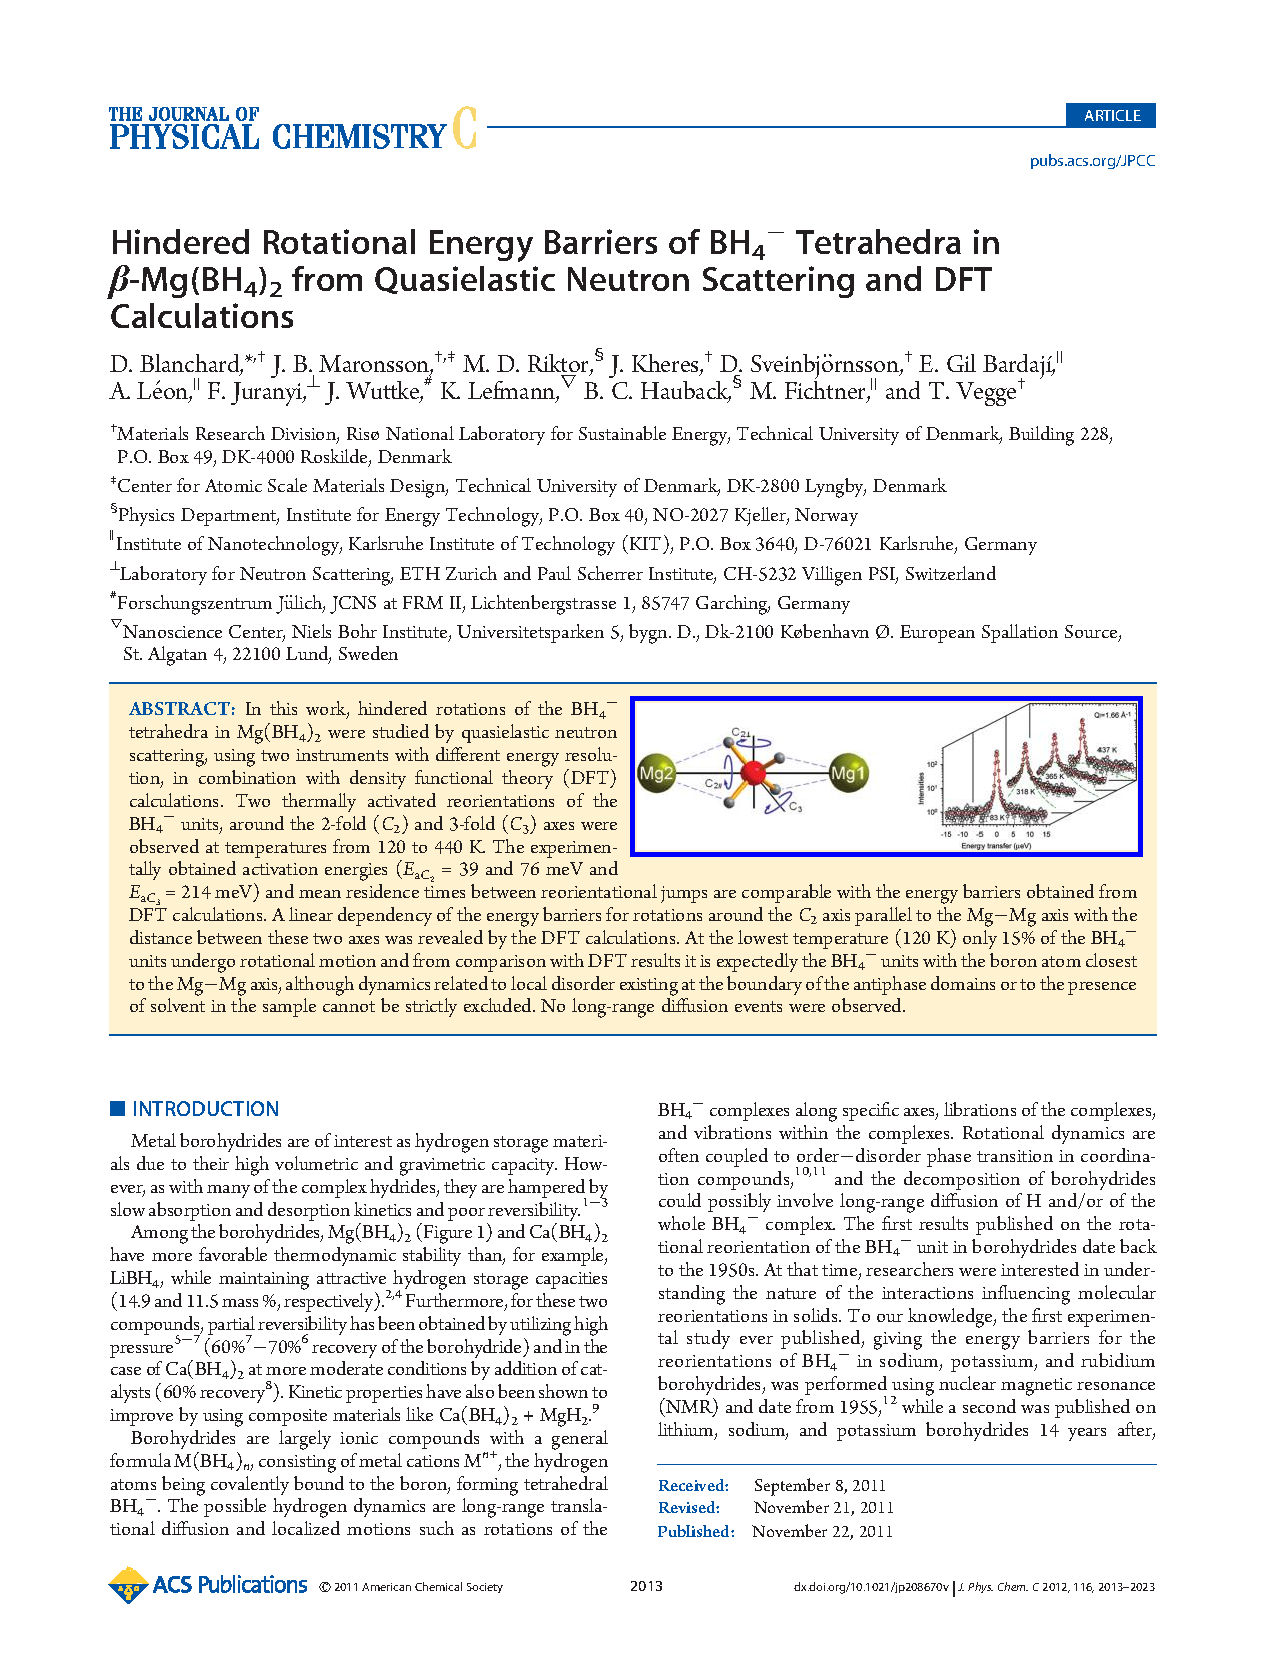
\includepdf[pages=1, addtotoc={1,chapter,0,Hindered Rotational Energy Barriers of \ce{BH4-} Tetrahedra in $\beta$-\ce{Mg(BH4)2} from Quasielastic Neutron Scattering and DFT Calculations,pap:magnesium}]{papers/magnesium.pdf}
%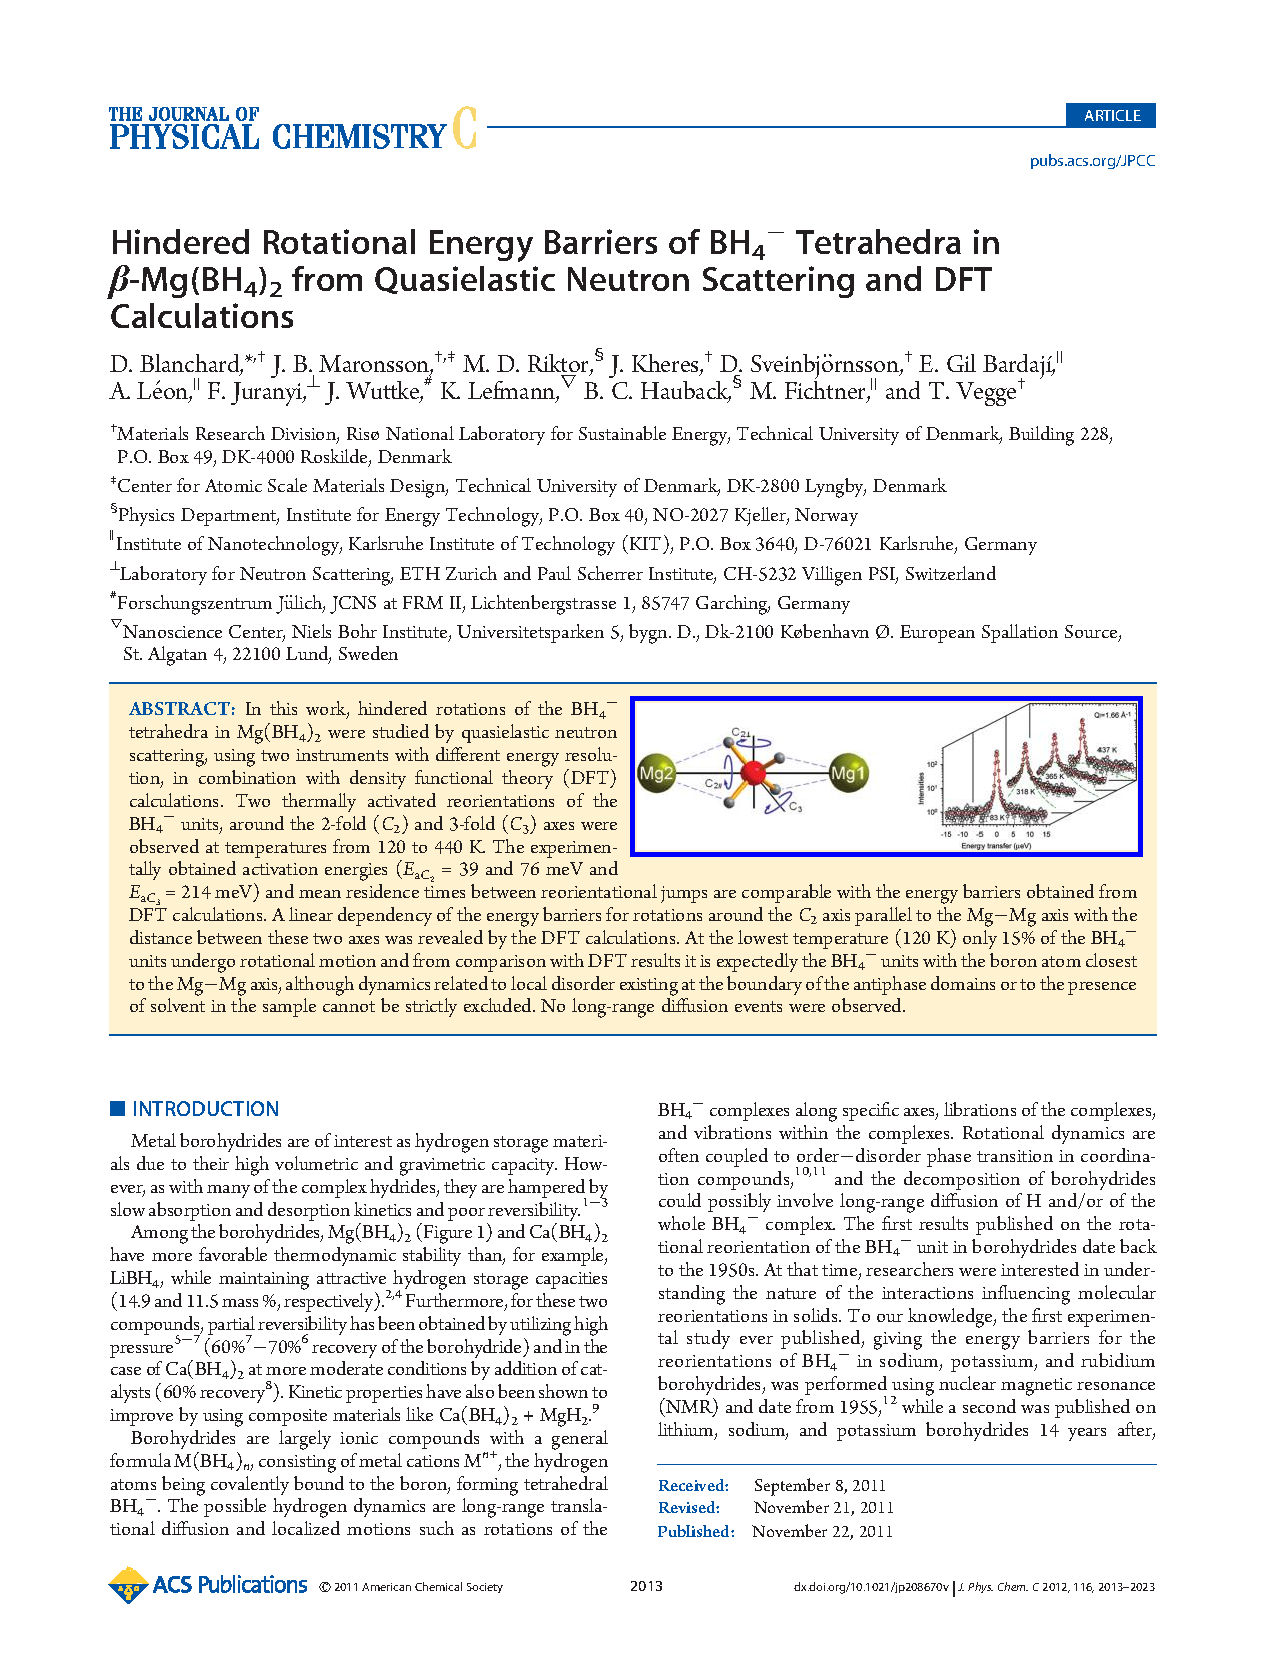
\includepdf[pages=-, openright, fitpaper, addtotoc={1,chapter,0,Hindered Rotational Energy Barriers of \ce{BH4-} Tetrahedra in $\beta$-\ce{Mg(BH4)2} from Quasielastic Neutron Scattering and DFT Calculations,pap:magnesium}]{papers/magnesium.pdf}

%\appchapter{A method for finding the ridge between saddle points applied to rare event rate estimates}
%\label{pap:second-order}
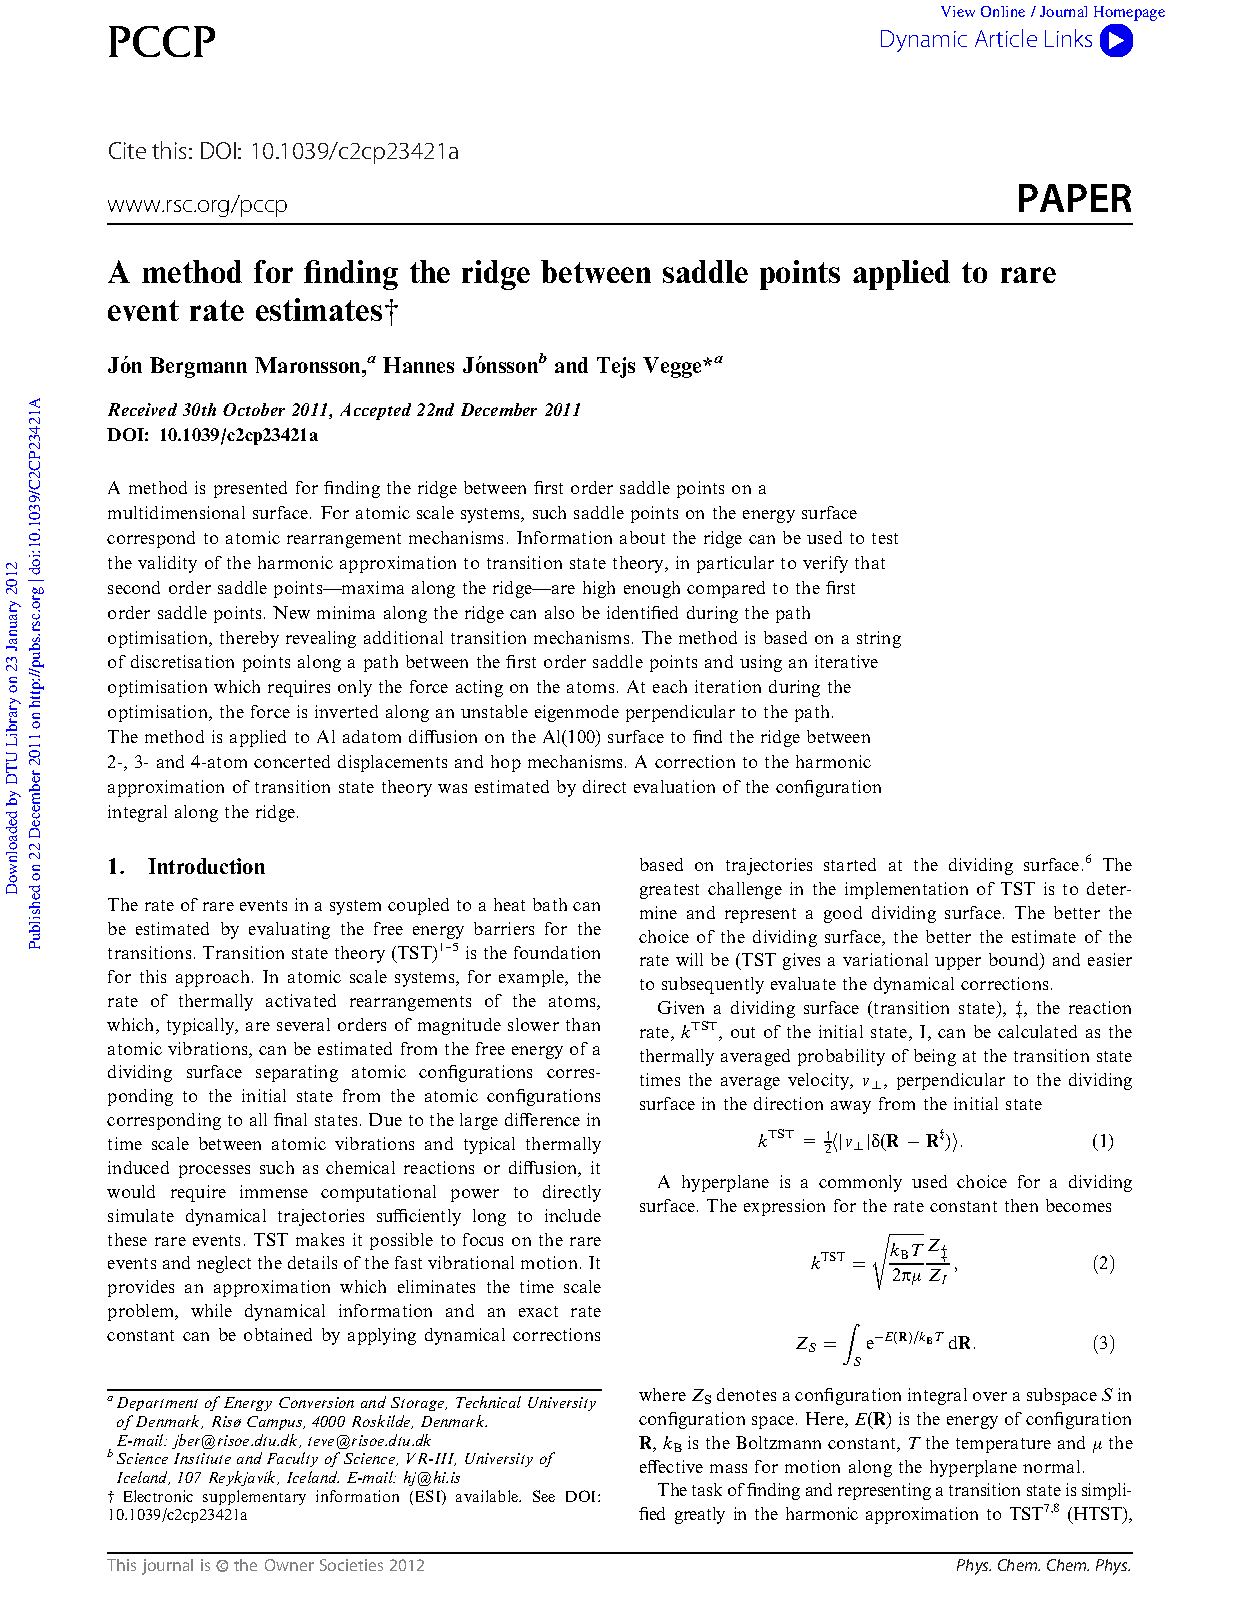
\includepdf[pages=1, addtotoc={1,chapter,0,A method for finding the ridge between saddle points applied to rare event rate estimates,pap:second-order}]{papers/second-order.pdf}
%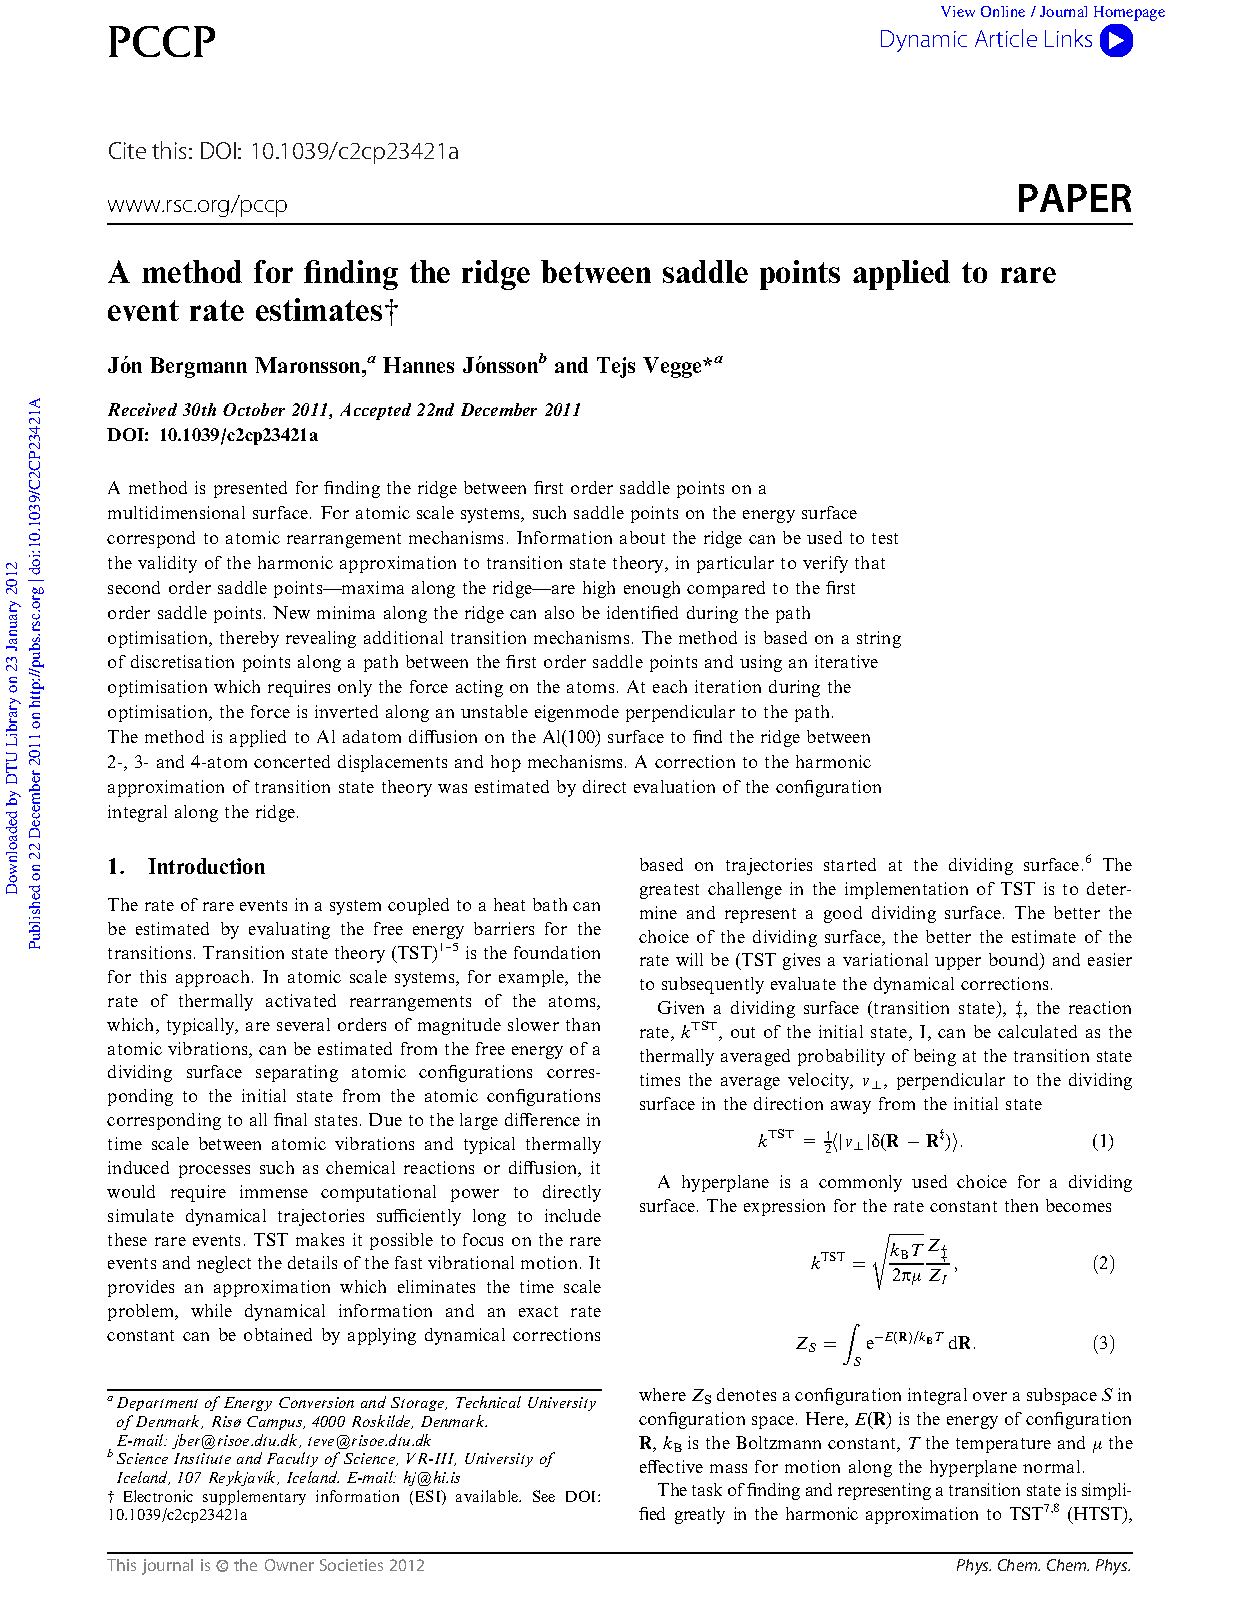
\includepdf[pages=-, openright, fitpaper, addtotoc={1,chapter,0,A method for finding the ridge between saddle points applied to rare event rate estimates,pap:second-order}]{papers/second-order.pdf}
